\chapter{Results}

In this chapter will be presented the results of the experiments \nameExperimentI{} and \nameExperimentII{}, along side with a discussion of the impact on the lift and similarity distributions of these experiments relative to the OT without the clustering.

\section{Experiment \nameExperimentI}

As seen on \ref{ch:experiment-i} this experiment was the one that creates sub-runs of the OT for each cluster in the portfolio. Also, it had to be created some heuristics to deal with clusters that did not have enough data to run. Using the "manually clustering", as discussed on \ref{ch:cluster-algorithm} the summary of the lift gain (how much the lift on the first decile increased or decreased relative to the OT without clustering) is presented on Table \ref{table:lift_gain_exp-i}. 

The cells are colored to better understand the gains. The green ones represent a positive gain, the light red ones represent a sightly negative gain, the dark red ones represent a considerable negative gain, the white represent that the lift did not change, and finally the orange ones are the outliers which were defined using the interquartile range rule \cite{upton1996understanding}. 

There are, also, some studies that are bolded. They represent the studies that brought up the hypothesis of this work, as discussed on the Introduction, they had two or more high density areas on the similarity distribution plot, meaning that, they can have more than one profile on their portfolio.

\begin{table}[h]
\centering
\begin{tabular}{|c|c|c|c|}
\hline
\textbf{Study} & \textbf{Lift Gain (\%)}        & \textbf{Study} & \textbf{Lift Gain (\%)}        \\ \hline
1              & \cellcolor[HTML]{ff514d}-12,09 & 15             & \cellcolor[HTML]{ff514d}-13,26 \\ \hline
2              & \cellcolor[HTML]{8ed08e}16,67  & \textbf{16}    & \cellcolor[HTML]{ff514d}-20,00 \\ \hline
3              & \cellcolor[HTML]{8ed08e}0,89   & \textbf{17}    & \cellcolor[HTML]{ffccc9}-4,28  \\ \hline
4              & 0,00                           & 18             & \cellcolor[HTML]{ff514d}-13,06 \\ \hline
5              & \cellcolor[HTML]{ffccc9}-0,14  & 19             & \cellcolor[HTML]{ff514d}-15,42 \\ \hline
6              & \cellcolor[HTML]{ff514d}-17,28 & 20             & \cellcolor[HTML]{8ed08e}0,57   \\ \hline
7              & \cellcolor[HTML]{ff514d}-12,44 & \textbf{21}    & \cellcolor[HTML]{ff514d}-33,95 \\ \hline
\textbf{8}     & \cellcolor[HTML]{ffccc9}-5,17  & 22             & 0,00                           \\ \hline
\textbf{9}     & \cellcolor[HTML]{ff514d}-27,78 & 23             & \cellcolor[HTML]{ff514d}-28,16 \\ \hline
\textbf{10}    & \cellcolor[HTML]{8ed08e}6,25   & 24             & \cellcolor[HTML]{ffce93}200,01 \\ \hline
11             & \cellcolor[HTML]{ff514d}-17,75 & \textbf{25}    & \cellcolor[HTML]{ff514d}-12,77 \\ \hline
12             & \cellcolor[HTML]{ffccc9}-1,01  & 26             & \cellcolor[HTML]{ff514d}-29,35 \\ \hline
13             & \cellcolor[HTML]{ff514d}-6,93  & 27             & \cellcolor[HTML]{ffccc9}-0,08  \\ \hline
14             & \cellcolor[HTML]{ffccc9}-1,16  &                &                                \\ \hline
\end{tabular}
\caption{Summary of the first-decile lift gains for Experiment \nameExperimentI}
\label{table:lift_gain_exp-i}
\end{table}

We can see that only 5 studies had positive impact on the lift, and one of them is an outlier. The majority of the studies had a negative impact - 6 of them were sightly negative and 14 worsened the lift considerably. It is important to notice that two studies did not present any changes on the lift with the clustering.

The Figure \ref{fig:lift-hist-plot-exp-i} shows a histogram of the lift gain for the studies excluding the outliers. We can see that the mean lift gain for \nameExperimentI{} is \textbf{-9.871 \%}.

\begin{figure}[h]
   \centering
   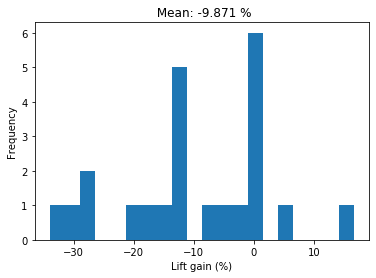
\includegraphics[width=\linewidth]{fig/ch4-lift-hist-plot-exp-i.png}
   \caption{Histogram plot of the studies' lift gain for experiment \nameExperimentI{}. Source: Author}
   \label{fig:lift-hist-plot-exp-i}
\end{figure}

\section{Experiment \nameExperimentII{}}

Now for the second experiment, which was the simple use of the clustering information as another feature. Using the same color scheme as Table \ref{table:lift_gain_exp-i}, Table \label{table:lift_gain_exp-ii} shows the summary of the lift gains for the experiment \nameExperimentII{}.

\begin{table}[h]
\centering
\begin{tabular}{|c|c|c|c|}
\hline
\textbf{Study} & \textbf{Lift Gain (\%)}        & \textbf{Study} & \textbf{Lift Gain (\%)}        \\ \hline
1              & \cellcolor[HTML]{8ed08e}4,40   & 15             & \cellcolor[HTML]{8ed08e}0,46   \\ \hline
2              & \cellcolor[HTML]{ff514d}-8,33  & \textbf{16}    & \cellcolor[HTML]{ff514d}-6,58  \\ \hline
3              & \cellcolor[HTML]{ffce93}23,65  & \textbf{17}    & \cellcolor[HTML]{ffce93}-46,08 \\ \hline
4              & 0,00                           & 18             & \cellcolor[HTML]{ffccc9}-1,87  \\ \hline
5              & \cellcolor[HTML]{8ed08e}1,49   & 19             & \cellcolor[HTML]{8ed08e}3,58   \\ \hline
6              & \cellcolor[HTML]{ffce93}-28,33 & 20             & \cellcolor[HTML]{ff514d}-11,28 \\ \hline
7              & \cellcolor[HTML]{8ed08e}12,50  & \textbf{21}    & \cellcolor[HTML]{ffccc9}-2,64  \\ \hline
\textbf{8}     & \cellcolor[HTML]{8ed08e}16,84  & 22             & \cellcolor[HTML]{8ed08e}1,23   \\ \hline
\textbf{9}     & \cellcolor[HTML]{8ed08e}12,80  & 23             & \cellcolor[HTML]{ffccc9}-0,14  \\ \hline
\textbf{10}    & \cellcolor[HTML]{8ed08e}18,59  & 24             & \cellcolor[HTML]{ffce93}300,02 \\ \hline
11             & \cellcolor[HTML]{ff514d}-7,84  & \textbf{25}    & \cellcolor[HTML]{8ed08e}4,90   \\ \hline
12             & \cellcolor[HTML]{ffccc9}-0,15  & 26             & \cellcolor[HTML]{ffccc9}-0,77  \\ \hline
13             & \cellcolor[HTML]{8ed08e}0,68   & 27             & \cellcolor[HTML]{8ed08e}1,21   \\ \hline
14             & \cellcolor[HTML]{8ed08e}7,30   &                &                                \\ \hline
\end{tabular}
\caption{Summary of the first-decile lift gains for Experiment \nameExperimentII}
\label{table:lift_gain_exp-ii}
\end{table}

We can see that, differently from \nameExperimentI{}, the majority of the studies had positive gain (16 studies, to be exactly). Only 4 studies were considerably worse on the lift gain and 5 sightly worse, a total of 9 studies. Only one study did not presented any change on the lift and, this time, 4 were outliers (2 positives and 2 negatives).

The Figure \ref{fig:lift-hist-plot-exp-ii} shows a histogram of the lift gain for the studies excluding the outliers. We see that the mean lift gain for \nameExperimentII{} is \textbf{2.016 \%}.

\begin{figure}[h]
   \centering
   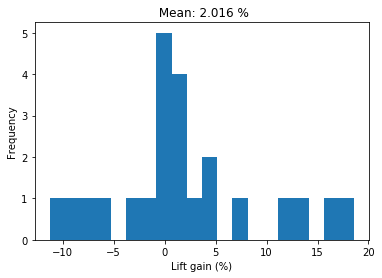
\includegraphics[width=\linewidth]{fig/ch4-lift-hist-plot-exp-ii.png}
   \caption{Histogram plot of the studies' lift gain for experiment \nameExperimentII{}. Source: Author}
   \label{fig:lift-hist-plot-exp-ii}
\end{figure}

\section{Similarity distributions}
\label{ch:simi-distis}

Now let us look at some of the similarity distributions plots for both experiments. These plots will have three curves: the market similarity in green, the holdout set in orange, and the portfolio in blue. Each topic of this section will address a group represented by the colors in the lift gain summary tables. 

\subsection{Studies with no change on the lift}

In both experiments there were studies that do not had any variation on the lift. \underline{Study 4} appeared on both. Figure \ref{fig:study-4-comparsion} shows the similarity distribution plots for Study 6. The first row is the run of the OT without the clustering, and the second row is with the clustering. On the left is presented the \nameExperimentI{} experiment and on the right \nameExperimentII{}. There is, also, on the information about the size of the sets in the study. This is a study with around 4600 companies on the portfolio (1100 are the Holdout set) and a market around 220 thousand companies, meaning that the portfolio correspond to approximately 1.5\% of the companies on the study.

\begin{figure}[h]
   \centering
   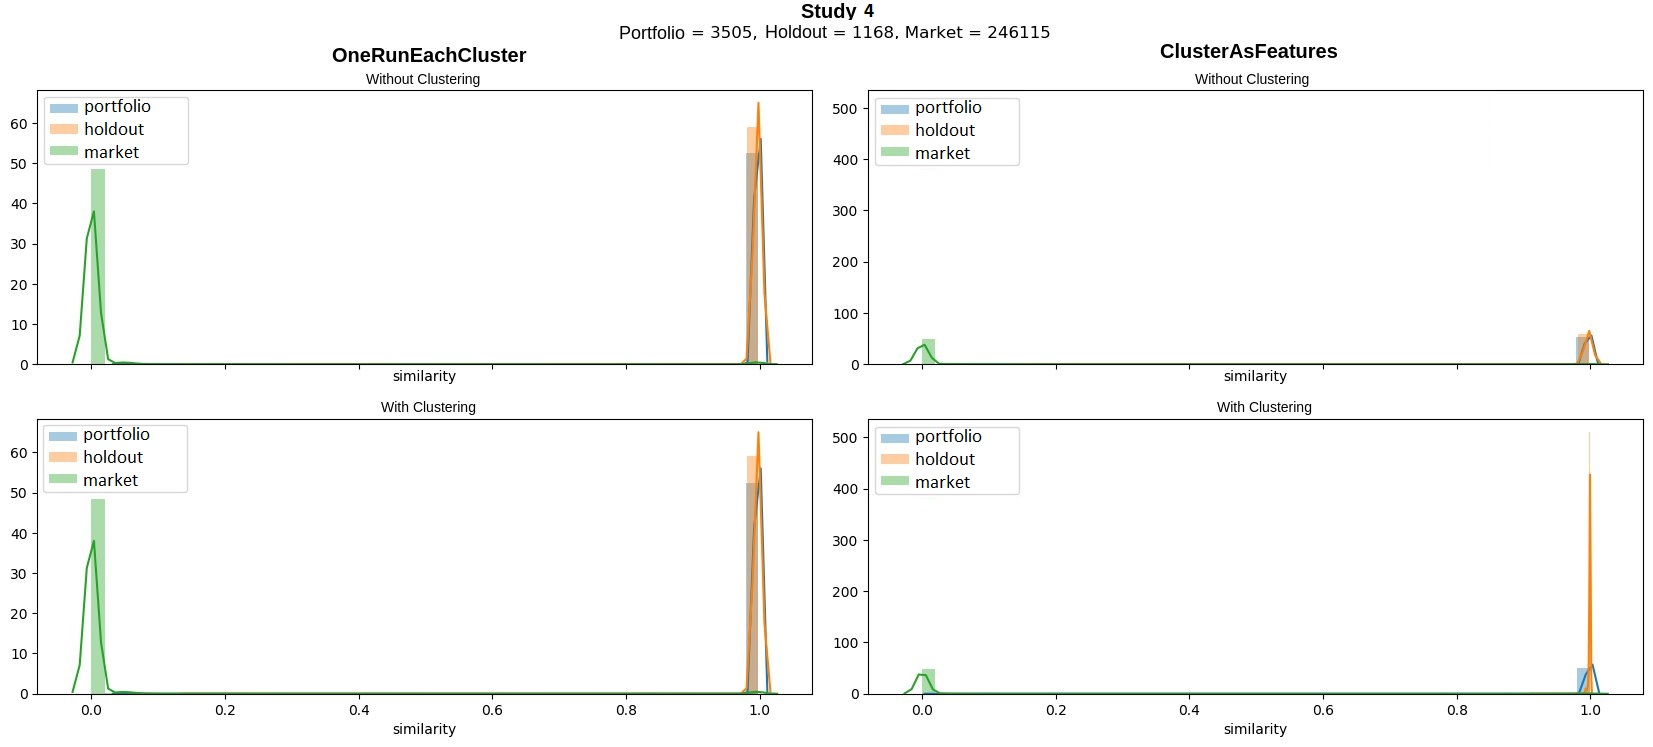
\includegraphics[width=\linewidth]{fig/ch4-study-4-comparsion.jpg}
   \caption{Similarity distribution plot for \underline{Study 4} for both experiments. Source: Author}
   \label{fig:study-4-comparsion}
\end{figure}

\begin{figure}[h]
   \centering
   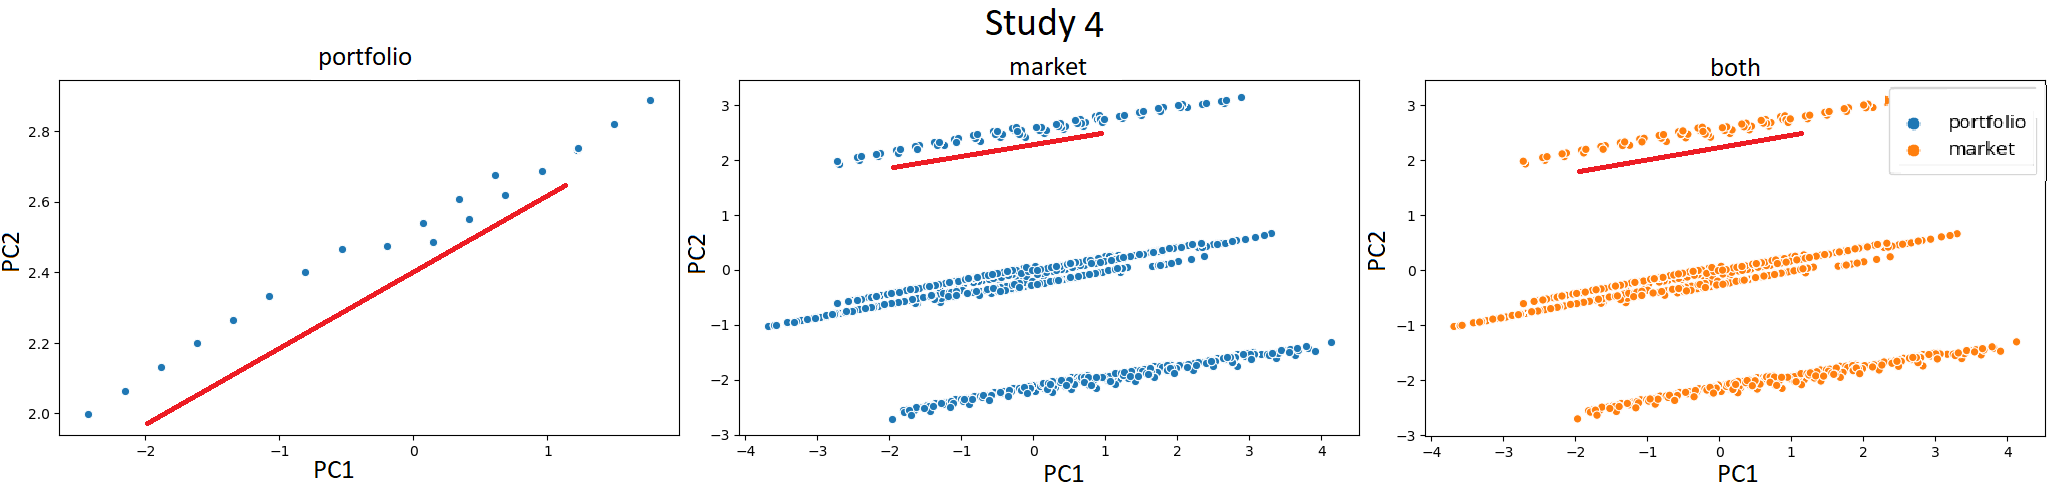
\includegraphics[width=\linewidth]{fig/ch4-study-4-pca-plot.png}
   \caption{PCA plot for \underline{Study 4}. The red line is the same on the three plots. Source: Author}
   \label{fig:study-4-pca-plot}
\end{figure}

We can see that on \nameExperimentI{} the similarity distributions with and without clustering are virtually the same. This is better understood when you look at the number of clusters in its portfolio. Figure \ref{fig:study-4-pca-plot} shows its PCA plot. There is only a single cluster on the portfolio, consequentially, the result of this cluster is the same of the aggregated output and, at the same time, the result without clustering.

On \nameExperimentII{}, however, there is a difference on the distributions between the with and without the clustering. Basically, the holdout set changed its distribution. In this experiment the OT scored this companies with really close scores, in other words, their standard deviation decreased. But, even though the scores of the companies (and possibly the ordering) of the holdout set changed, the lift kept the same because of the way to calculate this metric. The same number of companies (of the holdout set) on the first decile occurred in the run without the clustering and in with the clustering, thus the value of the lift is the same for both runs.

Another study that had a zero lift gain was \underline{Study 22}, in the \nameExperimentI{} experiment. Figure \ref{fig:study-22-clusters-simi-plot} shows the similarity distribution plots for the clusters' runs of this study.

\begin{figure}[h]
   \centering
   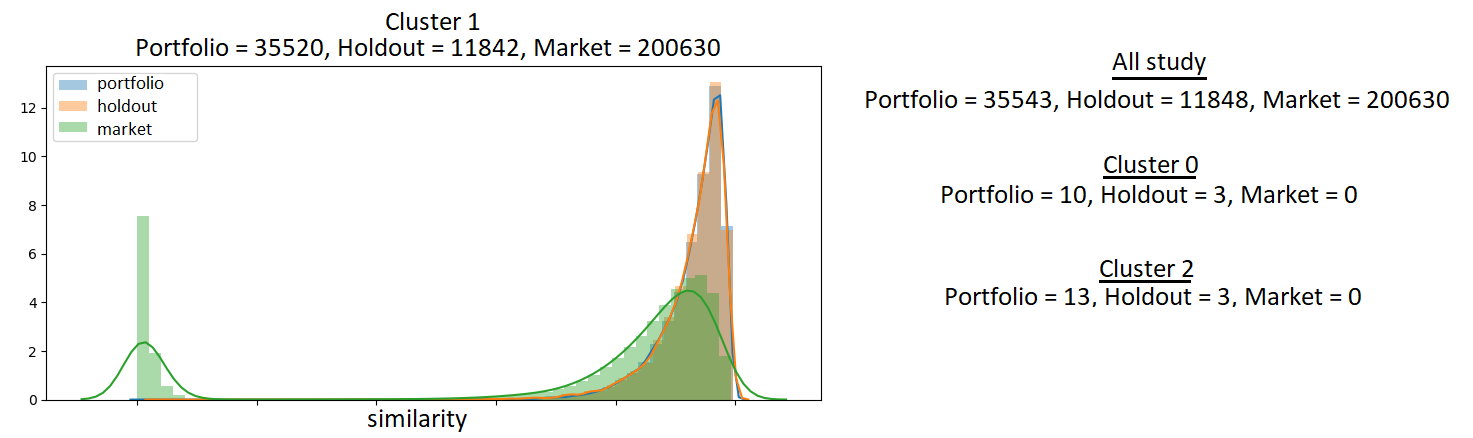
\includegraphics[width=\linewidth]{fig/ch4-study-22-clusters-simi-plot.png}
   \caption{Similarity distribution plot for the clusters' runs of \underline{Study 22} on experiment \nameExperimentI{}. Source: Author}
   \label{fig:study-22-clusters-simi-plot}
\end{figure}

Although this study has 3 clusters on the portfolio, only Cluster 1 has the minimum data to a valid run. Cluster 0 and Cluster 2 do not have companies on the Market, so the 16 companies of the former and 13 companies of latter were discarded. Since they represent less than 0.001 \% of the overall data of the study, the behavior is practically the same as Study 4, thus, for the same reason, the lift is the same for both runs (with and without clustering).

\subsection{Studies with marginal increase or decrease on the lift}
\label{ch:marginal-change}

Both experiments had studies that changed the lift in a minor way, positively and negatively. This studies improved or lowered the lift up to approximately 5\%. Studies \underline{3, and 20} and studies \underline{5, 12, 14, 17, and 27} are, respectively, examples of sightly improvement and reduction on the lift for the experiment \nameExperimentI{}. For experiment \nameExperimentII{} the studies are, respectively, studies \underline{5, 13, 15, 19, 22, 25, and}
\underline{27} and studies \underline{12, 18, 21, 23, and 26}.

All of these studies had the same prevalent behavior: the overall distributions of the three sets (portfolio, holdout, and market) before and after the clustering were almost the same. There is a small difference on the holdout distribution. Figures \ref{fig:study-5-marginal-increase-exp-2} and \ref{fig:study-12-marginal-decrease-exp-1} illustrate, respectively, examples of a small increase and decrease on the lift. In the former, the similarity distributions plot for \underline{Study 5} in experiment \nameExperimentII{}, and in the latter the same plot for \underline{Study 12} for experiment \nameExperimentI{}.

\begin{figure}[h]
   \centering
   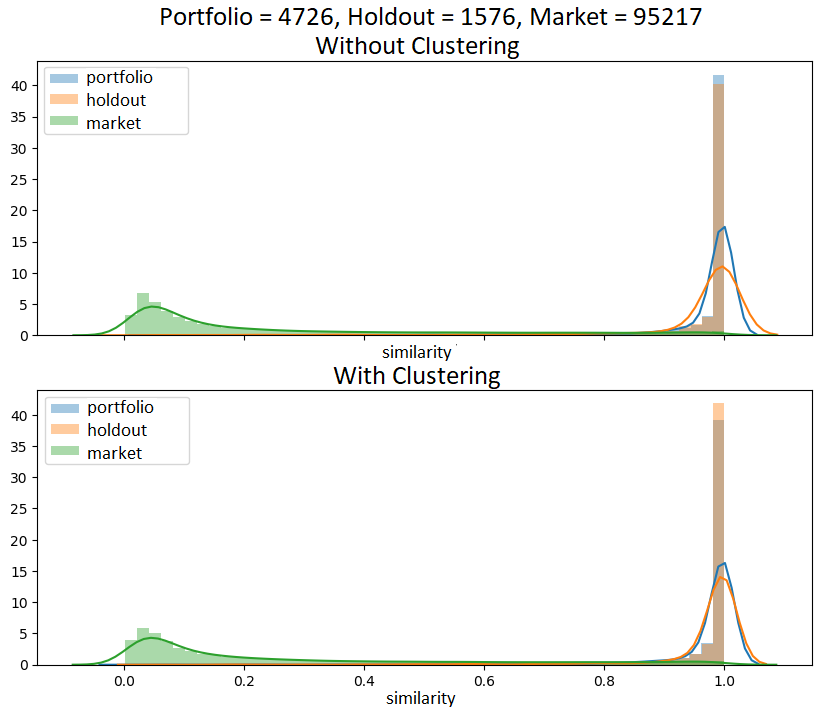
\includegraphics[width=7cm]{fig/ch4-study-5-marginal-increase-exp-2.png}
   \caption{Similarity distribution plot for \underline{Study 5} on experiment \nameExperimentII{}. An example of marginal increase on the lift. Source: Author}
   \label{fig:study-5-marginal-increase-exp-2}

   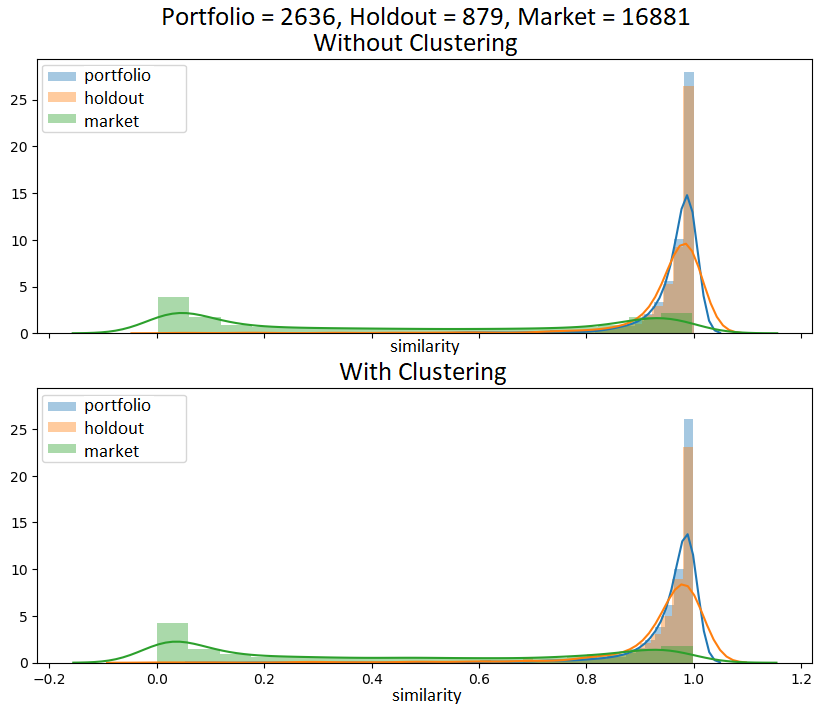
\includegraphics[width=7cm]{fig/ch4-study-12-marginal-decrease-exp-1.png}
   \caption{Similarity distribution plot for \underline{Study 12} on experiment \nameExperimentI{}. An example of marginal decrease on the lift. Source: Author}
   \label{fig:study-12-marginal-decrease-exp-1}
\end{figure}

We can notice that the peak near similarity 1 of the holdout set goes from approximately 37 to beyond 40 in Figure \ref{fig:study-5-marginal-increase-exp-2}. The opposite happens in Figure \ref{fig:study-12-marginal-decrease-exp-1}, the peak goes from almost 25 to 20.

\subsection{Studies with considerable increase or decrease on the lift}
\label{ch:considerable-change}

Most of the studies on both experiment had more than 5\% variation on the lift (positive and negative). In \nameExperimentI{}, 14 of them were negative (\underline{Studies: 1, 6, 7, 9, 11, 13, 15, 16, 18, 19, 21, 23, 25, 26}), and only \underline{Study 2} was positive. However, in experiment \nameExperimentII{}, 5 were positive (\underline{Studies: 7, 8, 9, 10, 14}) and 4 were negative (\underline{Studies: 2, 11, 16, 20}).

The behavior of the similarity distributions with the clustering follows the same idea as \ref{ch:marginal-change}, but with more exacerbate results. Figure \ref{fig:study-8-considerable-increase-exp-2} shows the similarity distributions with and without clustering for \underline{Study 8} in experiment \nameExperimentII{}, which is an example of a considerable increase on lift. In contrast, Figure \ref{fig:study-9-considerable-decrease-exp-1} displays the same plot for \underline{Study 9} in experiment \nameExperimentI{}, an example of considerable decrease on the lift.

\begin{figure}[h]
   \centering
   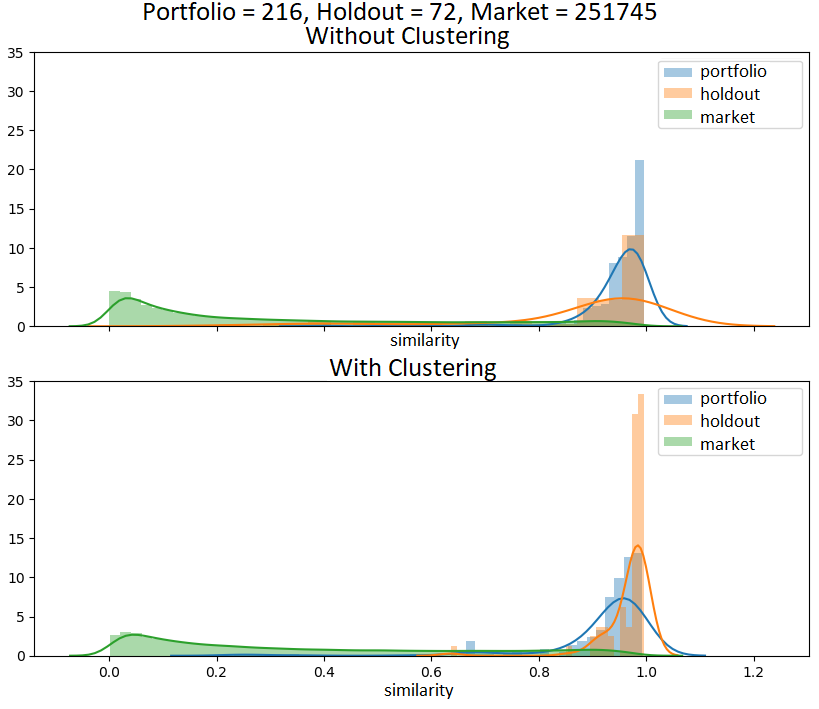
\includegraphics[width=7cm]{fig/ch4-study-8-considerable-increase-exp-2.png}
   \caption{Similarity distribution plot for \underline{Study 8} on experiment \nameExperimentII{}. An example of considerable increase on the lift. Source: Author}
   \label{fig:study-8-considerable-increase-exp-2}

   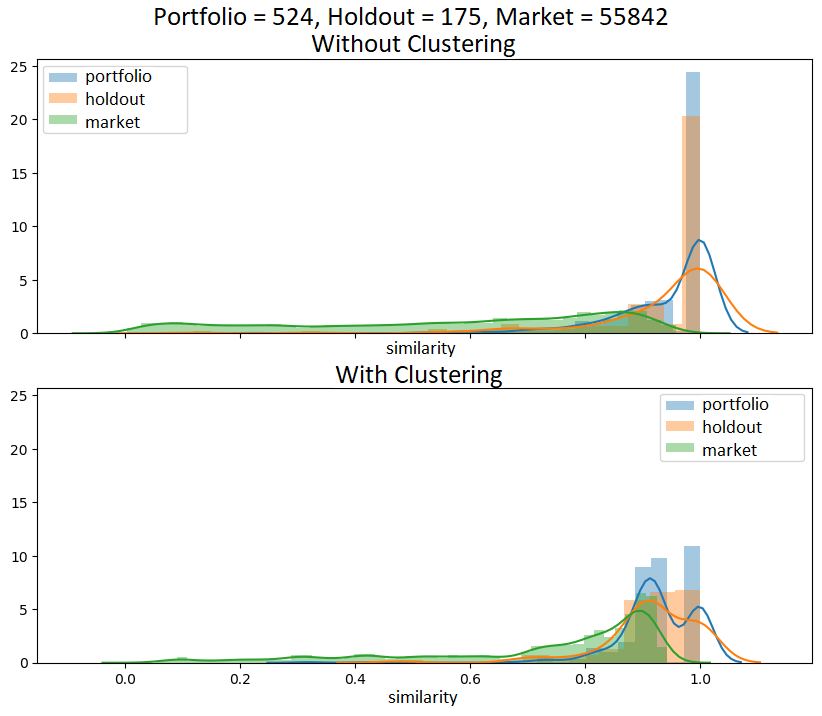
\includegraphics[width=7cm]{fig/ch4-study-9-considerable-decrease-exp-1.png}
   \caption{Similarity distribution plot for \underline{Study 9} on experiment \nameExperimentI{}. An example of considerable decrease on the lift. Source: Author}
   \label{fig:study-9-considerable-decrease-exp-1}
\end{figure}

Now the difference between the distributions, in these cases, is easier to spot. In Figure \ref{fig:study-8-considerable-increase-exp-2} we can see that the peak of the holdout set rose from 10 to more than 30. Consequentially, the curve became more thin, meaning that its variance decreased. The contrary to this, is showed on Figure \ref{fig:study-9-considerable-decrease-exp-1}. The peak of the holdout set distribution went from 20 to less than 10. Also, the portfolio distribution changed. Its single peak decreased by 15 units, and it was splitted in two peaks, one near 0.9 similarity and the other near similarity 1.0. This demonstrates that the OT was better at scoring the portfolio near similarity 1.0 without the clustering, which is the expected behavior. Moreover, the distribution of the market skewed to the right on this run, creating a high density area near 0.9 similarity. 

\subsection{Outliers studies}
\label{ch:outliers}

\underline{Study 24} was clearly the outlier of all studies. It got more than 200\% increase on the lift in both Experiments. In experiment \nameExperimentII{} more three studies were considered outliers due to the interquartile range rule - the lower and upper bound in this experiment were -14.77 \% and 18.62 \%, respectively. These studies had similar shift on the distributions as seen in \ref{ch:considerable-change}. Hence, just Study 24 similarity plot needs to be further delve into it. Figure \ref{fig:outlier-study-24-exp-2} exhibit the similarity distribution plot of this study in \nameExperimentII{}, and Figure \ref{fig:outlier-study-24-lift-exp-2} its lift plots, which contains the lifts of all deciles of the runs with and without the clustering.

\begin{figure}[h]
   \centering
   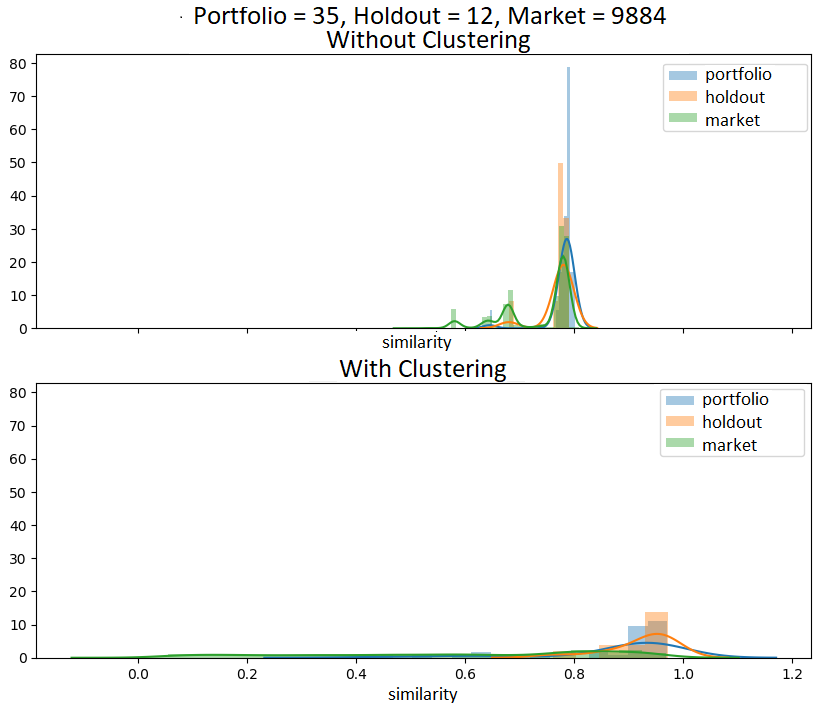
\includegraphics[width=7cm]{fig/ch4-outlier-study-24-exp-2.png}
   \caption{Similarity distribution plot for \underline{Study 24} on experiment \nameExperimentII{}. Source: Author}
   \label{fig:outlier-study-24-exp-2}

   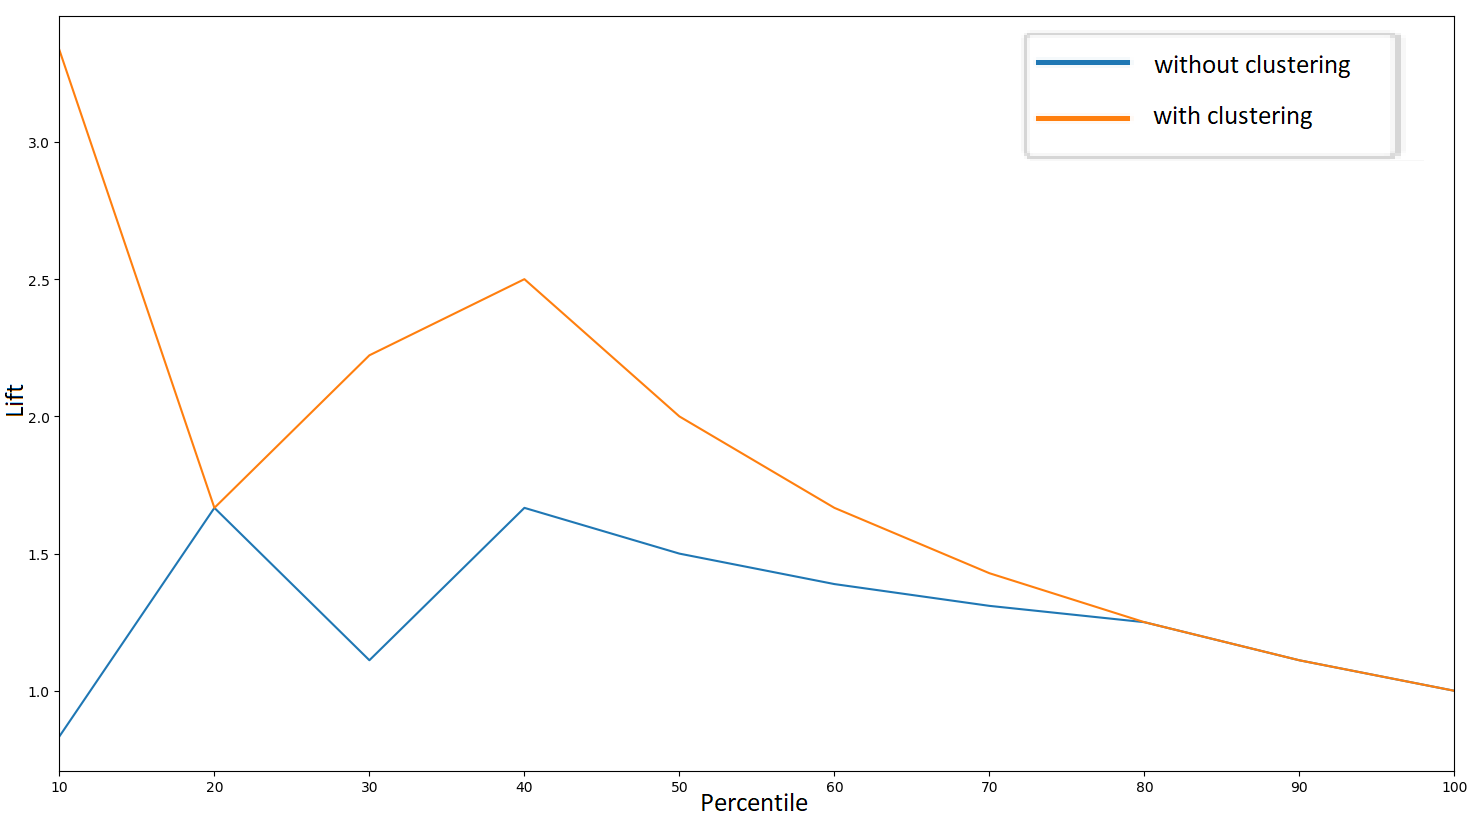
\includegraphics[width=7cm]{fig/ch4-outlier-study-24-lift-exp-2.png}
   \caption{Lift plot for \underline{Study 24} on experiment \nameExperimentII{}. Source: Author}
   \label{fig:outlier-study-24-lift-exp-2}
\end{figure}

The main aspect of this study is presented in Figure \ref{fig:outlier-study-24-exp-2}. There is the bizarre shape of the three distributions of the run without the clustering. All the data is bundled in three peaks with the highest one located at similarity 0.8. The OT could not even classify the portfolio of this study close to similarity 1.0. Moreover, the number of companies for each of the sets of the study is unbalanced. There are only 35 companies in the portfolio and 12 in the holdout set against a market with two orders of magnitude higher. This discrepancy can be one of the issues that led this study to have odd similarity distributions.

This issue is reinforced when we look at Figure \ref{fig:outlier-study-24-lift-exp-2}. The expected shape of a lift curve is in the form of a decreasing exponential, in other words, the lift of the decile on the left is greater than the one in the right, but this is not what happens on both runs of the experiment for this study. In the run with the clustering the lift of the second decile is lower than the fourth one. On top of that, the lift of the first decile in the run without the clustering is lower than 1.0. This, in practice, means that the sorting of the OT is worse than the random chance. So, in this case, the OT would be hindering the user.

With the clustering, the distributions skewed to right, with the holdout set being the closest to similarity 1.0. This explains why the lift of the first decile skyrocketed over 200\% in the run with the clustering.

Although the gap of the portfolio size and market size can be possible cause for this behavior, the real reason still unknown due to time constraints for this work. Other factors as: the features' data and how the user created this run (the filters applied) must be further investigate to completely solve this issue. For now, this study will be considered an outlier.

\subsection{Studies that had multiple profiles in its portfolio}

The last group of studies to be analyzed are the bolded ones in both tables (\ref{table:lift_gain_exp-i} and \ref{table:lift_gain_exp-ii}). These are the studies that sparked the idea of clustering the portfolio before running the OT. However, most of them did not had the expected behavior. Let us use one example that illustrate this result. Figure \ref{fig:bump-study-25} displays the similarity distributions plots for \underline{Study 25} for the runs in experiment \nameExperimentII{}. 

Study 25 is a study with a positive lift gain, that is, the performance of the study improved. However, looking at Figure \ref{fig:bump-study-25} we notice that the three high density areas of the portfolio distributions in the run without the clustering are preserved in the run with the clustering. We expected that each one of these peaks - that could be a cluster - would shift to right, close to similarity 1.0, since the performance improved. 

If we take a look at each clusters' similarity distributions plot we can see more clues for this behavior. Figure \ref{fig:study-25-clusters-pca} shows these plots (I), alongside the clusters' sets sizes of the runs that did not had enough data (II) and its PCA plot with the portfolio and the market (III). There are 5 cluster in the portfolio, but only two (Cluster 3 and 4) had a pair with the market. In these cases we see that they did not present a "one peak area" in the portfolio. Cluster 4 has two peaks: one near similarity 1.0 and the other near 0.8, and Cluster 3 two close peaks near similarity 0.9. The other clusters with not enough data (0, 1, 2), the portfolio and holdout sets correspond to approximately 10\% of the study portfolio size. This is a small portion of the data and it only affects \nameExperimentI{}, after all, in \nameExperimentII{} there is no cluster pairing, since this information is used as a feature.

The outcome of these studies demonstrate that, perhaps, \textbf{our initial hypothesis is not on point}. There still other analysis to be done, such as, analyzing the companies from the similarity perspective, for instance, seeing what the companies in the high density area near similarity 0.9 of some study have in common. These new perspectives emerged as the work was being developed. However, because of the time constraint, they could not be prioritized in this proof of concept. 
\begin{figure}[h]
   \centering
   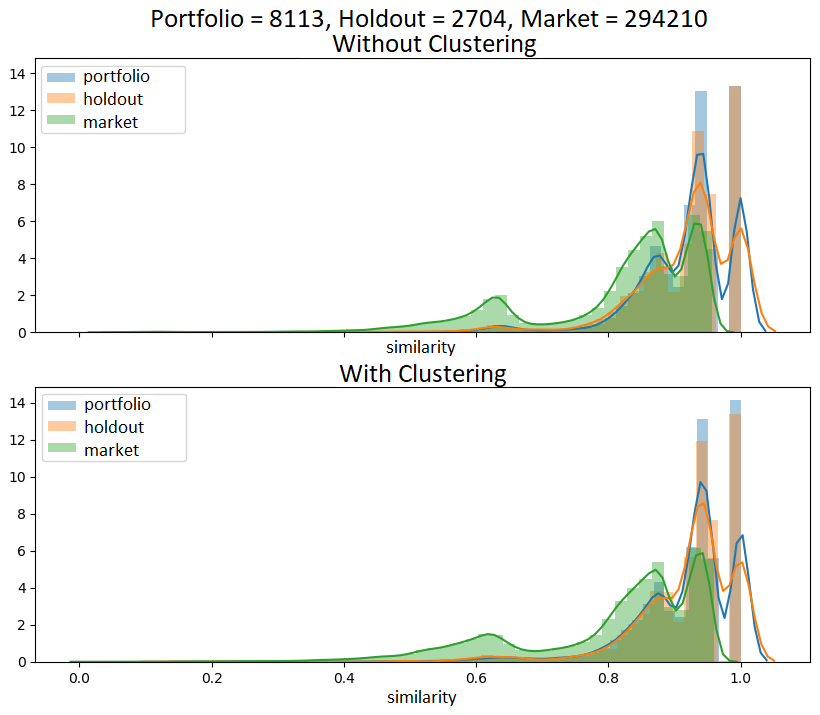
\includegraphics[width=7cm]{fig/ch4-bump-study-25.png}
   \caption{Similarity distribution plot for \underline{Study 25} on experiment \nameExperimentII{}. An example of study with multiple high density areas in the portfolio. Source: Author}
   \label{fig:bump-study-25}

   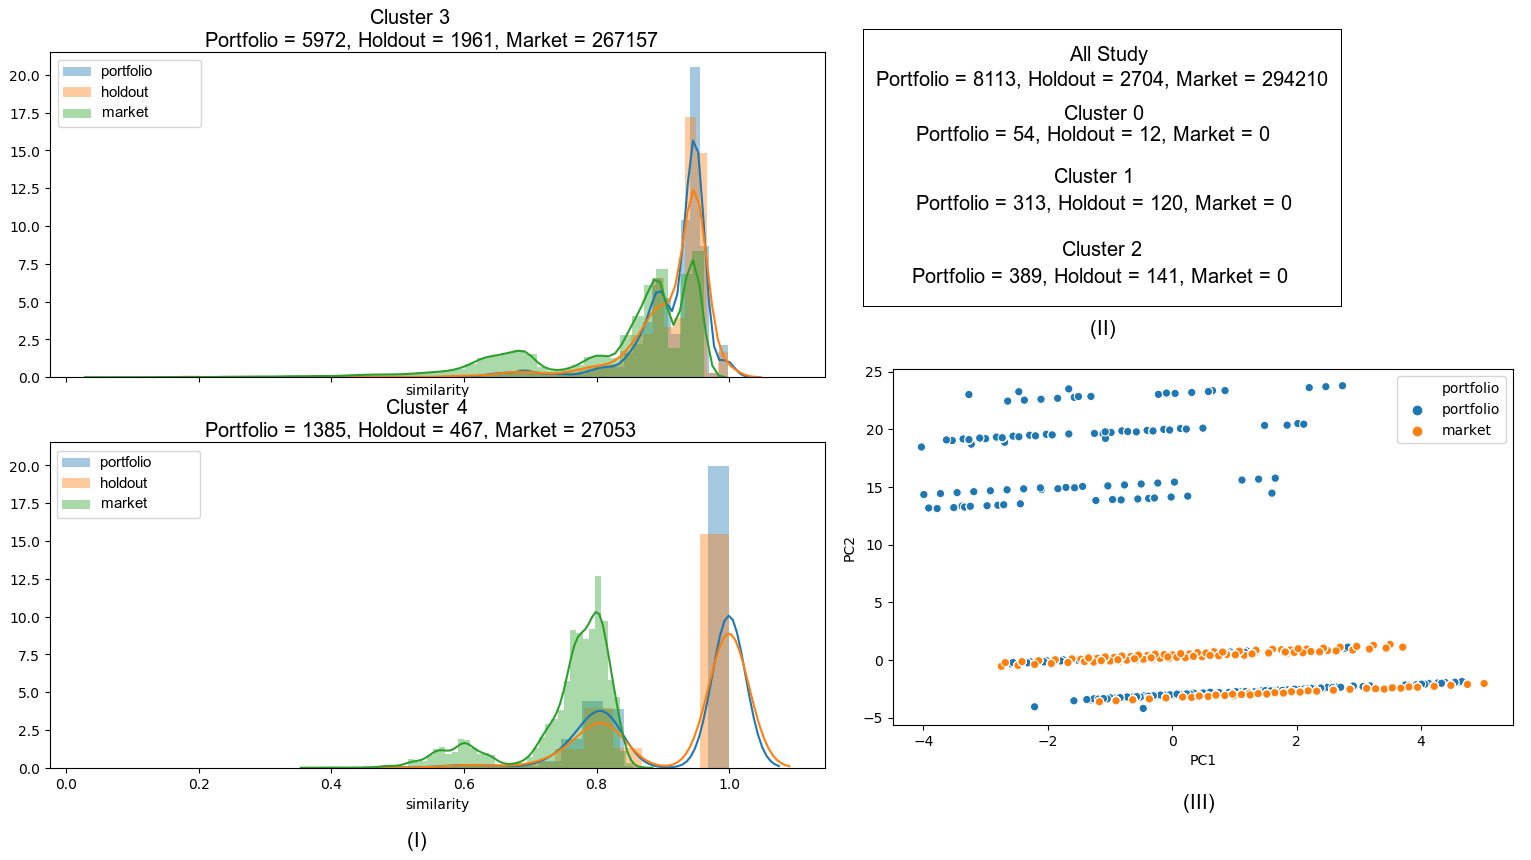
\includegraphics[width=\linewidth]{fig/ch4-study-25-clusters-pca.png}
   \caption{Clusters' similarity plots for \underline{Study 25} in experiment \nameExperimentI{} (I). The study's set sizes on the clusters that did not have enough data to a valid run (II). PCA plot for \underline{Study 25} with portfolio and market data. Source: Author}
   \label{fig:study-25-clusters-pca}
\end{figure}

\subsection{Other study worth mentioning}

There is another study that is not in one of the specifics lift-gain groups aforementioned, but its analysis of the similarity distribution is worth it to be considered. Figure \ref{fig:worth-mentioning-study-7} shows the similarity distribution plots for \underline{Study 7} in the experiment \nameExperimentII{}. This study had a lift gain of 12.5\%, so its performance improved, thus the expected impact in the distributions, as seen in the other studies of the same group before, is the holdout set increase its peak near similarity 1.0 or to shift to this region when the distribution is located more on the left of the axis. Nonetheless, the opposite happens in this study. In Figure \ref{fig:worth-mentioning-study-7}, we see that the distributions keep its shape but shifted from similarity 1.0 to around 0.85. But since the holdout distribution stayed more in the right, in the first decile there are more companies from the holdout set, hence the increase on the lift

The cause of this shift was not investigated. But the main point of mentioning this study is to raise the awareness of the OT's team in the choice of metrics. This example indicate that only the lift is not enough to verify the output of the OT. As seen throughout section \ref{ch:simi-distis}, the lift and the similarity distribution plot are correlated, specially the distribution of the holdout set. Still, the lift is a metric of \underline{performance} and the similarity distribution plot shows the \underline{consistency} of the study. The shift of Study 7 was not critical, but if the similarity that the distributions went was 0.3 instead of the 0.85, the recommendations would not make sense for the OT's user due to its lack of consistency. That is why a new metric, that take into account consistency and performance, should be included in the overall benchmark of the studies.

\begin{figure}[h]
   \centering
   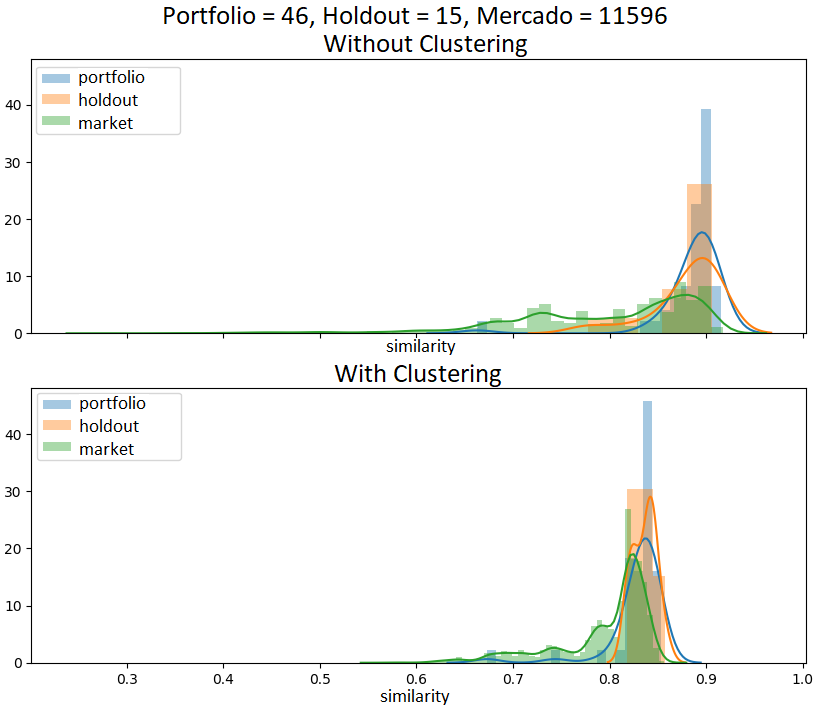
\includegraphics[width=7cm]{fig/ch4-worth-mentioning-study-7.png}
   \caption{Similarity distribution plot for \underline{Study 7} on experiment \nameExperimentII{}. Lift increased but the curves skewed to the left. Source: Author}
   \label{fig:worth-mentioning-study-7}
\end{figure}

\section{Experiment \nameExperimentII{} with other clustering algorithms}

The poor performance of the studies in experiment \nameExperimentI{}, which as the mean lift gain of -9.871\%, made the team of the OT to not proceed the testing of the clustering with this experiment. Although \nameExperimentII{} had a positive mean lift gain of +2.016\%, it was conducted with the "manual clustering". Thus, it was determined to oversee the results of this experiment with the other clustering algorithms previously presented in Figure \ref{fig:clustering-studies}. Figure \ref{fig:other-cluster-algo} shows the histogram of the lift gains of the re-runs for \nameExperimentII{} with \underline{KMeans} (top left), \underline{Gaussian Mixture} (top right), and \underline{Bayesian Gaussian Mixture} (below).

We notice that none of them reached the lift gain of the "manual clustering". The closest one was the Gaussian Mixture with 1.13\%. The other two resided below 1\% (0.8 for KMeans and approximately 0.3 for Bayesian Gaussian Mixture). The outcome of these results fortify the strategy of cluster the studies manually, meaning that the groups in the PCA plots make sense, at least in the performance perspective of the OT. 

Despite of this confirmation on the strategy adopted by the team, this is not feasible for the OT, since it is impossible to the system run in production with human interference during the leads scoring. The clustering done manually could be use as a success criteria for other clustering algorithms, but that would turn the type of problem to a classification, due to the presence of the labels. This new viewpoint opens the possibility to test the algorithms that classify data by defining a line or plane that separate the classes, for instance, Support Vector Machine (SVM) \cite{suykens1999least}. Although interesting, this approach was not included in this PoC.

Another alternative to improve the performance in experiment \nameExperimentII{} without the manual clustering, is to tweak the hyper-parameters of the Gaussian Mixture and see if it the lift gain approaches the achieved mark of 2\%. For instance, in the Scikit-learn Python package, this algorithm has up to seven different hyper parameters that go from initialization, weights settings up to convergence settings \cite{scikit-learn}. Again, this was not part of the scope of the PoC.

\begin{figure}[h]
   \centering
   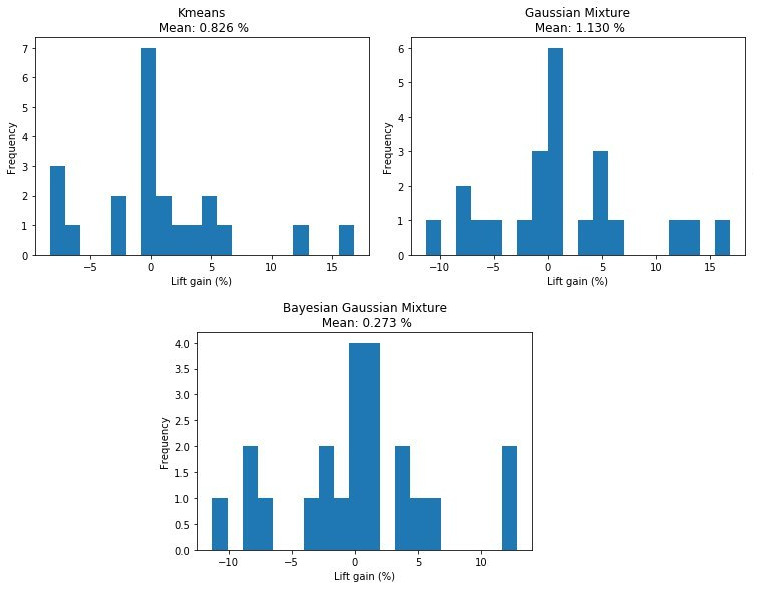
\includegraphics[width=8cm]{fig/ch4-other-cluster-algo.png}
   \caption{Lift gain histogram without outliers of other clustering algorithm runs for experiment \nameExperimentII{}. In the top left is the KMeans, in the top right is the Gaussian Mixture and below the Bayesian Gaussian Mixture. Source: Author}
   \label{fig:other-cluster-algo}
\end{figure}
 
